\cleardoublepage
\begin{titlepage}
	{\centering
	\vspace{3cm}
	{\Huge\sffamily\bfseries Forord \par} \vspace{0.5cm}}
	\noindent
	
	% Fed tekst 	\bfseries
	% Kursiv		\itshape
	% Ingen serif 	\sffamily
	% Størrelse		\large \Large \LARGE \huge \Huge
	% Slut paragraf \par
	% Vertikalt rum \vspace{1cm}
	% Centrer 		\centering
	
	{\large\bfseries Hello world! \par}
	
	Din computer er et kraftfuldt værktøj, som kan mange ting. Man kan kun løse problemer med værktøjer man forstår, så en grundig forståelse af teknologiens redskaber bliver essentiel for fremtidens samfund. Både for alle som arbejder med færdige programmer, men også for os som udvikler dem. 
	
	Mens du sidder og læser denne bog, foretager din mobiltelefon tusindvis af beregninger. Udviklingen er uundgåelig, og med den opstår nye problemer som du kan være med til at løse. 
	
	Du skal nu til at tage et skridt videre. Vi vil forsøge at hjælpe dig med at lære programmeringsværktøjet at kende.
	Husk, det er ikke vigtigt at du forstår alle koncepterne i bogen med det samme, det er ikke sådan man lærer.
	Det tager tid at forstå tankegangen bag. Det skal øves.
	Så tag jeres tid, og hav det sjovt, for sådan lærer man bedst.
	Vi håber at vi med denne bog hjælper jer godt på vej til at lære at programmere og giver jer en ny måde at analysere problemer i støder på, også andre steder end foran en computer.
	
	TL;DR: Denne bog er en introduktion til Java programmering og app-udvikling til Android. 
	
	GLHF
	
	- Fagligt team
	
	{\centering
	{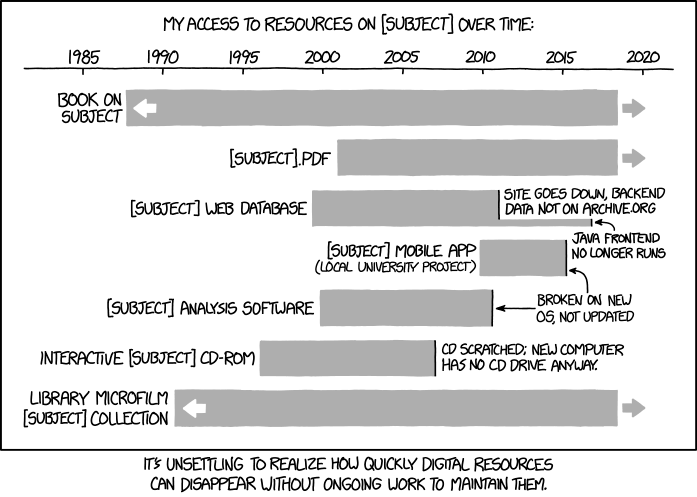
\includegraphics[width=7cm]{digital_resource_lifespan}\\
		\tiny \url{https://xkcd.com/1909/} \par} \vspace{0.5cm}}
\end{titlepage}
